\section{Internal Block Diagram - BMS}
Due to the complexity of the Battery Management System its interconnectivity has been visualized on a separate Internal Block Diagram. The result is seen below.

\begin{figure}[H]
	\centering
	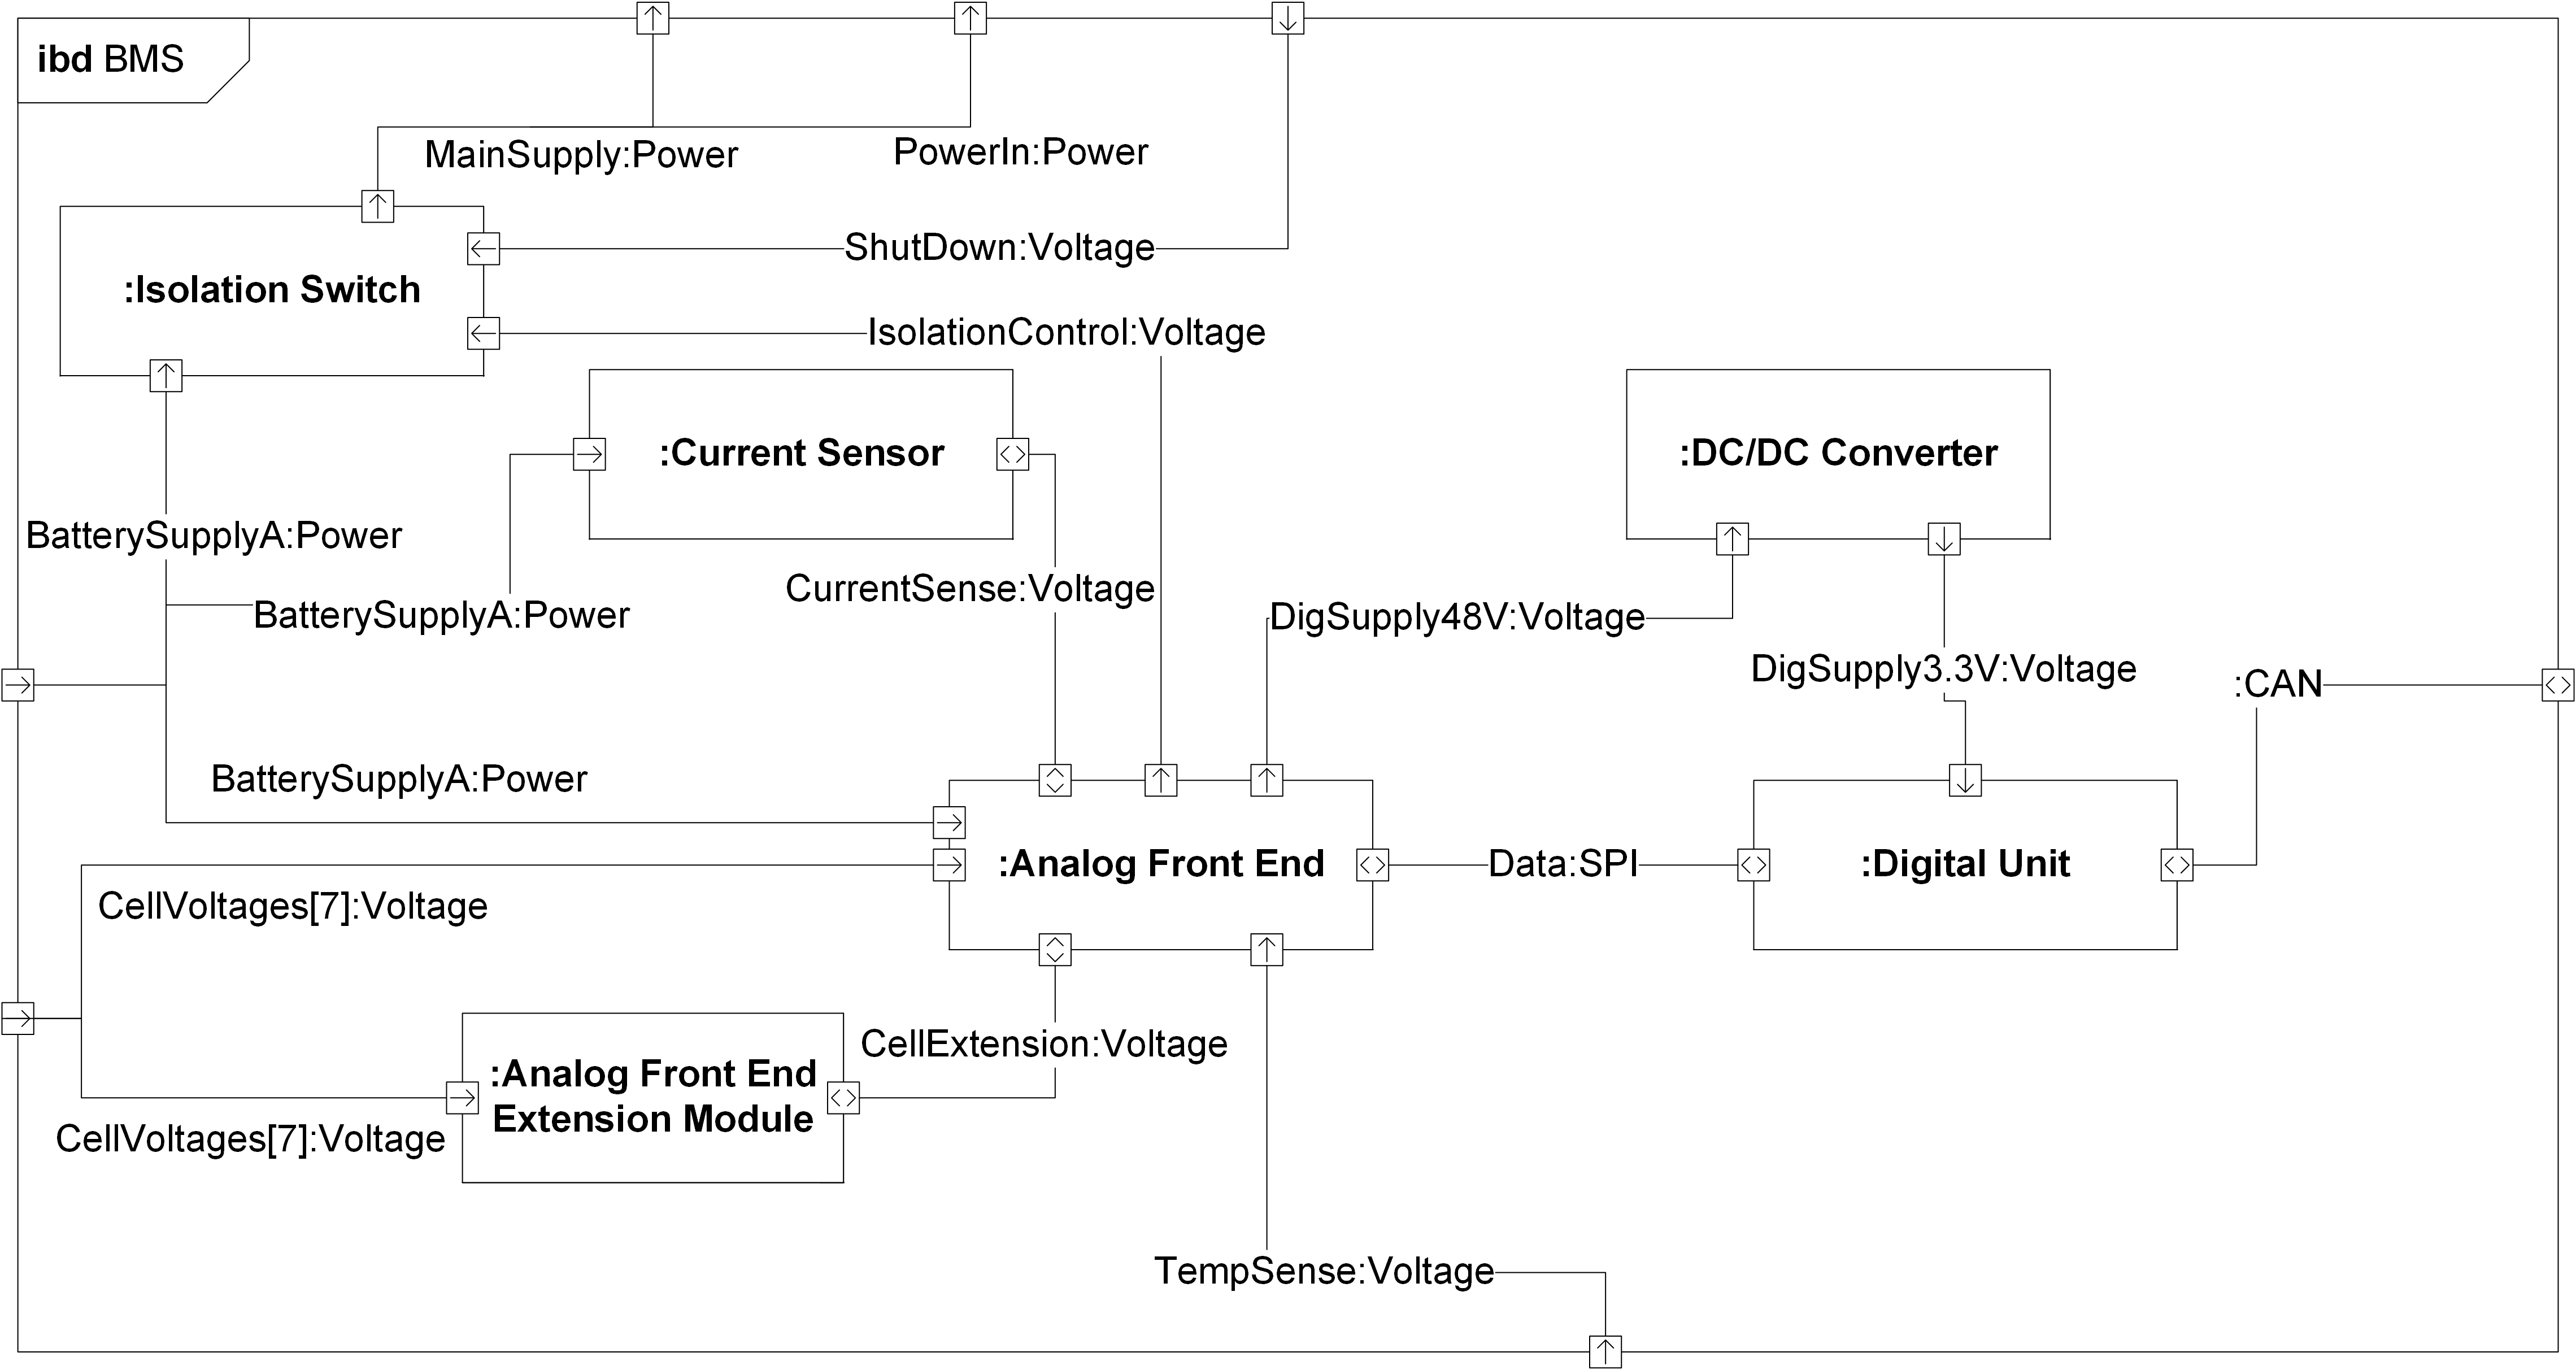
\includegraphics[width=1\linewidth]{Architecture/Diagrams/IBD_BMS}
	\caption{IBD for AU2's Management System}
	\label{fig:IBD_BMS}
\end{figure}

\section{Signal description - BMS}
The signals and protocols used to communicate between the blocks in BMS are specified in this section.

\textbf{Block :BMS}\\
Block interface description:
\begin{itemize}
	\item \textbf{ShutDown:Voltage}\\
	Direction: [External] $\rightarrow$ [Isolation Switch]\\
	Description: Shuts down the system if a change in the voltage-level is measured from 48 V to 0 V. This happens when the corresponding Emergency Shutdown Switch(Emergency System) is pressed.
	\item \textbf{MainSupply:Power \& PowerIn:Power}\\
	Direction: [Isolation Switch] $\rightarrow$ [External]\\
	Description: The power from the battery which is delivered through the relay to the remaining electrical systems in the car. 
	\item \textbf{:CAN}\\
	Direction: [External] $\leftrightarrow$ [Digital Unit]\\
	Description: CAN-communication with a computer in order to gain information about various variables.
	\item \textbf{BatterySupplyA:Power}\\
	Direction: [External] $\rightarrow$ [Current Sensor]\\
	Description: Power coming from the battery that is protected by a fuse.
	\item \textbf{CellVoltages:Voltage}\\
	Direction: [External] $\rightarrow$ [Analog Front End \& Analog Front End Extension Module]\\
	Description: Voltages that indicate the voltage of the individual cells.
	\item \textbf{TempSense:Voltage}\\
	Direction: [External] $\rightarrow$ [Analog Front End]\\
	Description: A voltage which is proportional to the battery's temperature.
\end{itemize}

\textbf{Block :Current Sensor}\\
Block interface description:
\begin{itemize}
	\item \textbf{BatterySupplyA:Power}\\
	Direction: [External] $\rightarrow$ [Current Sensor]\\
	Description: Power coming from the battery that is protected by a fuse.
	\item \textbf{CurrentSense:Voltage}\\
	Direction: [Current Sensor] $\rightarrow$ [Analog Front End]\\
	Description: A voltage which is proportional to the output current from the battery.
\end{itemize}

\textbf{Block :Analog Frontend}\\
Block interface description:
\begin{itemize}
	\item \textbf{CellVoltages:Voltage}\\
	Direction: [External] $\rightarrow$ [Analog Front End]\\
	Description: Voltages that indicate the voltage of the individual cells.
	\item \textbf{CurrentSense:Voltage}\\
	Direction: [Current Sensor] $\rightarrow$ [Analog Front End]\\
	Description: A voltage which is proportional to the output current from the battery.
	\item \textbf{IsolationControl:Voltage}\\
	Direction: [Analog Front End] $\rightarrow$ [Isolation Switch]\\
	Description: Wire that the Analog Front End uses to control the Isolation Switch. If and error occurs on the BMS the IsolationControl will follow the ShutDown connection.
	\item \textbf{CellExtension:Voltage}\\
	Direction: [Analog Front End Extension Module] $\rightarrow$ [Analog Front End]\\
	Description: Signals containing information about cell voltages from the Extension Module.
	\item \textbf{BatterySupplyA:Voltage}\\
	Direction: [External] $\rightarrow$ [Analog Front End]\\
	Description: Power coming from the battery that is protected by a fuse.
	\item \textbf{Error:SPI}\\
	Direction: [Analog Front End] $\leftrightarrow$ [Digital Unit]\\
	Description: Sends the measured analog data to the digital unit in order to be sent to a computer.
	\item \textbf{DigSupply48V:Voltage}\\
	Direction: [Analog Front End] $\rightarrow$ [DC/DC Converter]\\
	Description: Supply voltage from the Analog Front End which has to be converted to be used on the Digital Unit.
	\item \textbf{TempSense:Voltage}\\
	Direction: [External] $\rightarrow$ [Analog Front End]\\
	Description: A voltage which is proportional to the battery's temperature.
\end{itemize}

\textbf{Block :Isolation Switch}\\
Block interface description:
\begin{itemize}
	\item \textbf{BatterySupplyA:Voltage}\\
	Direction: [External] $\rightarrow$ [Isolation Switch]\\
	Description: Power coming from the battery that is protected by a fuse.
	\item \textbf{MainSupply:Power \& PowerIn:Power}\\
	Direction: [Isolation Switch] $\rightarrow$ [External]\\
	Description: The power from the battery which is delivered through the relay to the remaining electrical systems in the car. 
	\item \textbf{ShutDown:Voltage}\\
	Direction: [External] $\rightarrow$ [Isolation Switch]\\
	Description: Shuts down the system if a change in the voltage-level is measured from 48 V to 0 V. This happens when the corresponding Emergency Shutdown Switch(Emergency System) is pressed.
	\item \textbf{IsolationControl:Voltage}\\
	Direction: [Analog Front End] $\rightarrow$ [Isolation Switch]\\
	Description: Wire that the Analog Front End uses to control the Isolation Switch. If and error occurs on the BMS the IsolationControl will follow the ShutDown connection.  
\end{itemize}

\textbf{Block :DC/DC Converter}\\
Block interface description:
\begin{itemize}
	\item \textbf{DigSupply48V:Voltage}\\
	Direction: [Analog Front End] $\rightarrow$ [DC/DC Converter]\\
	Description: Supply voltage from the Analog Front End which has to be converted to be used on the Digital Unit.
	\item \textbf{DigSupply3.3V:Voltage}\\
	Direction: [DC/DC Converter] $\rightarrow$ [Digital Unit]\\
	Description: A converted voltage to 3.3V which supplies circuits in the Digital Unit. 
\end{itemize}

\textbf{Block :Analog Front End Extension Module}\\
Block interface description:
\begin{itemize}
	\item \textbf{CellVoltages:Voltage}\\
	Direction: [External] $\rightarrow$ [Analog Front End Extension Module]\\
	Description: Voltages that indicate the voltage of the individual cells.
	\item \textbf{CellExtension:Voltage}\\
	Direction: [Analog Front End Extension Module] $\rightarrow$ [Analog Front End]\\
	Description: Signals containing information about cell voltages from the Extension Module. 
\end{itemize}

\textbf{Block :Digital Unit}\\
Block interface description:
\begin{itemize}
	\item \textbf{Error:SPI}\\
	Direction: [Analog Front End] $\leftrightarrow$ [Digital Unit]\\
	Description: Sends the measured analog data to the Digital Unit in order to be sent to a computer via CAN later.
	\item \textbf{:CAN}\\
	Direction: [External] $\leftrightarrow$ [Digital Unit]\\
	Description: CAN-communication with a computer in order to gain information about various variables measured.
	\item \textbf{DigSupply3.3:Voltage}\\
	Direction: [DC/DC Converter] $\rightarrow$ [Digital Unit]\\
	Description: A converted voltage to 3.3V which supplies circuits in the Digital Unit. 
\end{itemize}

